\tikzstyle{wavey}=[decorate,decoration={coil, aspect=-.5, post length=1mm, segment length=1mm, pre length=2mm},
shorten <= -.8pt,shorten >= -0.8pt]

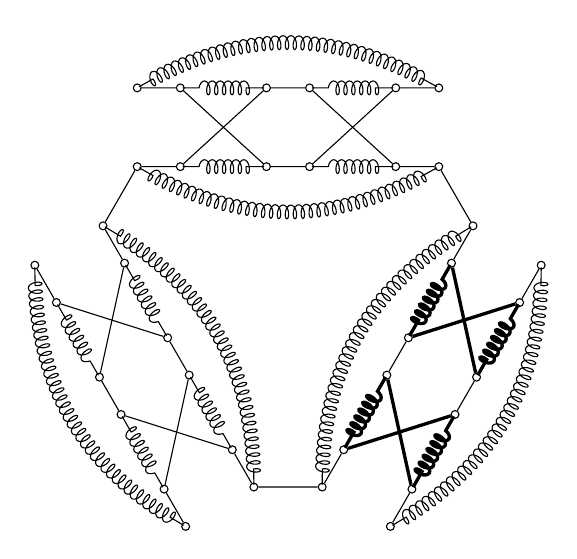
\begin{tikzpicture}[rotate=20,scale=0.5,
    vertex/.style={
        draw,
        circle, 
        inner sep=.0pt, 
        minimum size=0.1cm},
    every edge/.append style={}]
    \def\radius{5}
    \def\gap{1} 
    
    
    \pgfmathsetmacro\x{\radius * cos(0)}
    \pgfmathsetmacro\y{\radius * sin(0)}
    \node[vertex] (v1) at (\x,\y) {};
    
    \pgfmathsetmacro\xvFourteen{\radius * cos(260)}
    \pgfmathsetmacro\yvFourteen{\radius * sin(260)}
    \node[vertex] (v14) at (\xvFourteen, \yvFourteen) {};
    
    \node[vertex] (v15) at ({\xvFourteen + (1/7) * (\x - \xvFourteen)}, {\yvFourteen + (1/7) * (\y - \yvFourteen)}) {};
    \node[vertex] (v16) at ({\xvFourteen + (3/7) * (\x - \xvFourteen)}, {\yvFourteen + (3/7) * (\y - \yvFourteen)}) {};
    \node[vertex] (v17) at ({\xvFourteen + (4/7) * (\x - \xvFourteen)}, {\yvFourteen + (4/7) * (\y - \yvFourteen)}) {};
    \node[vertex] (v18) at ({\xvFourteen + (6/7) * (\x - \xvFourteen)}, {\yvFourteen + (6/7) * (\y - \yvFourteen)}) {};
    
    
    \pgfmathsetmacro\dx{\x - \xvFourteen}
    \pgfmathsetmacro\dy{\y - \yvFourteen}
    \pgfmathsetmacro\len{sqrt(\dx*\dx + \dy*\dy)}
    \pgfmathsetmacro\nx{\dy / \len} 
    \pgfmathsetmacro\ny{-\dx / \len} 
    
    
    \node[vertex] (mv1) at ({\x + 2*\gap*\nx}, {\y + 2*\gap*\ny}) {};
    \node[vertex] (mv14) at ({\xvFourteen + 2*\gap*\nx}, {\yvFourteen + 2*\gap*\ny}) {};
    \node[vertex] (mv15) at ({(\xvFourteen + (1/7) * (\x - \xvFourteen)) + 2*\gap*\nx}, 
                              {(\yvFourteen + (1/7) * (\y - \yvFourteen)) + 2*\gap*\ny}) {};
    \node[vertex] (mv16) at ({(\xvFourteen + (3/7) * (\x - \xvFourteen)) + 2*\gap*\nx}, 
                              {(\yvFourteen + (3/7) * (\y - \yvFourteen)) + 2*\gap*\ny}) {};
    \node[vertex] (mv17) at ({(\xvFourteen + (4/7) * (\x - \xvFourteen)) + 2*\gap*\nx}, 
                              {(\yvFourteen + (4/7) * (\y - \yvFourteen)) + 2*\gap*\ny}) {};
    \node[vertex] (mv18) at ({(\xvFourteen + (6/7) * (\x - \xvFourteen)) + 2*\gap*\nx}, 
                              {(\yvFourteen + (6/7) * (\y - \yvFourteen)) + 2*\gap*\ny}) {};
    
    
    \draw (v14) -- (v15);
    \draw[very thick, wavey] (v15) -- (v16); 
    \draw (v16) -- (v17);
    \draw[very thick, wavey] (v17) -- (v18); 
    \draw (v18) -- (v1);

    
    \draw[wavey] (mv1) to[bend left=30] (mv14);
    \draw (mv14) -- (mv15);
    \draw[very thick, wavey] (mv15) -- (mv16); 
    \draw (mv16) -- (mv17);
    \draw[very thick, wavey] (mv17) -- (mv18); 
    \draw (mv18) -- (mv1);

    
    \pgfmathsetmacro\xvTwo{\radius * cos(20)}
    \pgfmathsetmacro\yvTwo{\radius * sin(20)}
    \node[vertex] (v2) at (\xvTwo, \yvTwo) {};
    
    \pgfmathsetmacro\xvSeven{\radius * cos(120)}
    \pgfmathsetmacro\yvSeven{\radius * sin(120)}
    \node[vertex] (v7) at (\xvSeven, \yvSeven) {};
    
    \node[vertex] (v3) at ({\xvTwo + (1/7) * (\xvSeven - \xvTwo)}, {\yvTwo + (1/7) * (\yvSeven - \yvTwo)}) {};
    \node[vertex] (v4) at ({\xvTwo + (3/7) * (\xvSeven - \xvTwo)}, {\yvTwo + (3/7) * (\yvSeven - \yvTwo)}) {};
    \node[vertex] (v5) at ({\xvTwo + (4/7) * (\xvSeven - \xvTwo)}, {\yvTwo + (4/7) * (\yvSeven - \yvTwo)}) {};
    \node[vertex] (v6) at ({\xvTwo + (6/7) * (\xvSeven - \xvTwo)}, {\yvTwo + (6/7) * (\yvSeven - \yvTwo)}) {};

    
    \pgfmathsetmacro\dx{\xvSeven - \xvTwo}
    \pgfmathsetmacro\dy{\yvSeven - \yvTwo}
    \pgfmathsetmacro\len{sqrt(\dx*\dx + \dy*\dy)}
    \pgfmathsetmacro\nx{\dy / \len} 
    \pgfmathsetmacro\ny{-\dx / \len} 
    
    
    \node[vertex] (mv2) at ({\xvTwo + 2*\gap*\nx}, {\yvTwo + 2*\gap*\ny}) {};
    \node[vertex] (mv7) at ({\xvSeven + 2*\gap*\nx}, {\yvSeven + 2*\gap*\ny}) {};
    \node[vertex] (mv3) at ({(\xvTwo + (1/7) * (\xvSeven - \xvTwo)) + 2*\gap*\nx}, 
                                {(\yvTwo + (1/7) * (\yvSeven - \yvTwo)) + 2*\gap*\ny}) {};
    \node[vertex] (mv4) at ({(\xvTwo + (3/7) * (\xvSeven - \xvTwo)) + 2*\gap*\nx}, 
                                {(\yvTwo + (3/7) * (\yvSeven - \yvTwo)) + 2*\gap*\ny}) {};
    \node[vertex] (mv5) at ({(\xvTwo + (4/7) * (\xvSeven - \xvTwo)) + 2*\gap*\nx}, 
                                {(\yvTwo + (4/7) * (\yvSeven - \yvTwo)) + 2*\gap*\ny}) {};
    \node[vertex] (mv6) at ({(\xvTwo + (6/7) * (\xvSeven - \xvTwo)) + 2*\gap*\nx}, 
                                {(\yvTwo + (6/7) * (\yvSeven - \yvTwo)) + 2*\gap*\ny}) {};

    \draw[wavey] (mv2) to[bend right=30] (mv7);
    \draw (mv2) -- (mv3); 
    \draw[wavey] (mv3) -- (mv4); 
    \draw (mv4) -- (mv5);
    \draw[wavey] (mv5) -- (mv6); 
    \draw (mv6) -- (mv7);

    \pgfmathsetmacro\xvEight{\radius * cos(140)}
    \pgfmathsetmacro\yvEight{\radius * sin(140)}
    \node[vertex] (v8) at (\xvEight, \yvEight) {};

    \pgfmathsetmacro\xvThirteen{\radius * cos(240)}
    \pgfmathsetmacro\yvThirteen{\radius * sin(240)}
    \node[vertex] (v13) at (\xvThirteen, \yvThirteen) {};

    \node[vertex] (v9) at ({\xvEight + (1/7) * (\xvThirteen - \xvEight)}, {\yvEight + (1/7) * (\yvThirteen - \yvEight)}) {};
    \node[vertex] (v10) at ({\xvEight + (3/7) * (\xvThirteen - \xvEight)}, {\yvEight + (3/7) * (\yvThirteen - \yvEight)}) {};
    \node[vertex] (v11) at ({\xvEight + (4/7) * (\xvThirteen - \xvEight)}, {\yvEight + (4/7) * (\yvThirteen - \yvEight)}) {};
    \node[vertex] (v12) at ({\xvEight + (6/7) * (\xvThirteen - \xvEight)}, {\yvEight + (6/7) * (\yvThirteen - \yvEight)}) {};
    
    
    \pgfmathsetmacro\dx{\xvThirteen - \xvEight}
    \pgfmathsetmacro\dy{\yvThirteen - \yvEight}
    \pgfmathsetmacro\len{sqrt(\dx*\dx + \dy*\dy)}
    \pgfmathsetmacro\nx{\dy / \len} 
    \pgfmathsetmacro\ny{-\dx / \len} 
    
    
    \node[vertex] (mv8) at ({\xvEight + 2*\gap*\nx}, {\yvEight + 2*\gap*\ny}) {};
    \node[vertex] (mv13) at ({\xvThirteen + 2*\gap*\nx}, {\yvThirteen + 2*\gap*\ny}) {};
    \node[vertex] (mv9) at ({(\xvEight + (1/7) * (\xvThirteen - \xvEight)) + 2*\gap*\nx}, 
                             {(\yvEight + (1/7) * (\yvThirteen - \yvEight)) + 2*\gap*\ny}) {};
    \node[vertex] (mv10) at ({(\xvEight + (3/7) * (\xvThirteen - \xvEight)) + 2*\gap*\nx}, 
                              {(\yvEight + (3/7) * (\yvThirteen - \yvEight)) + 2*\gap*\ny}) {};
    \node[vertex] (mv11) at ({(\xvEight + (4/7) * (\xvThirteen - \xvEight)) + 2*\gap*\nx}, 
                              {(\yvEight + (4/7) * (\yvThirteen - \yvEight)) + 2*\gap*\ny}) {};
    \node[vertex] (mv12) at ({(\xvEight + (6/7) * (\xvThirteen - \xvEight)) + 2*\gap*\nx}, 
                              {(\yvEight + (6/7) * (\yvThirteen - \yvEight)) + 2*\gap*\ny}) {};

    \draw[wavey] (mv8) to[bend right=30] (mv13);
    \draw (mv8) -- (mv9);
    \draw[wavey] (mv9) -- (mv10); 
    \draw (mv10) -- (mv11);
    \draw[wavey] (mv11) -- (mv12); 
    \draw (mv12) -- (mv13);  

    
    \draw (v1) -- (v2);
    \draw (v2) -- (v3); 
    \draw[wavey] (v3) -- (v4); 
    \draw (v4) -- (v5);
    \draw[wavey] (v5) -- (v6); 
    \draw (v6) -- (v7);
    \draw (v7) -- (v8); 
    \draw (v8) -- (v9);
    \draw[wavey] (v9) -- (v10); 
    \draw (v10) -- (v11);
    \draw[wavey] (v11) -- (v12); 
    \draw (v12) -- (v13);
    \draw (v13) -- (v14); 
    \draw[wavey] (v1) to[bend right=30] (v14);
    \draw[wavey] (v2) to[bend left=30] (v7);
    \draw[wavey] (v8) to[bend left=30] (v13);

    \draw (mv3) -- (v4);
    \draw (mv4) -- (v3);
    \draw (mv5) -- (v6);
    \draw (mv6) -- (v5);

    \draw (mv9) -- (v10);
    \draw (mv10) -- (v9);
    \draw (mv11) -- (v12);
    \draw (mv12) -- (v11);

    \draw[very thick] (mv15) -- (v16);
    \draw[very thick] (mv16) -- (v15);
    \draw[very thick] (mv17) -- (v18);
    \draw[very thick] (mv18) -- (v17);
\end{tikzpicture}